
\documentclass{beamer}
\usepackage[utf8]{inputenc}

\usetheme{Madrid}
\usecolortheme{default}
\usepackage{amsmath,amssymb,amsfonts,amsthm}
\usepackage{txfonts}
\usepackage{tkz-euclide}
\usepackage{listings}
\usepackage{adjustbox}
\usepackage{array}
\usepackage{tabularx}
\usepackage{gvv}
\usepackage{lmodern}
\usepackage{circuitikz}
\usepackage{tikz}
\usepackage{graphicx}

\setbeamertemplate{page number in head/foot}[totalframenumber]

\usepackage{tcolorbox}
\tcbuselibrary{minted,breakable,xparse,skins}



\definecolor{bg}{gray}{0.95}
\DeclareTCBListing{mintedbox}{O{}m!O{}}{%
  breakable=true,
  listing engine=minted,
  listing only,
  minted language=#2,
  minted style=default,
  minted options={%
    linenos,
    gobble=0,
    breaklines=true,
    breakafter=,,
    fontsize=\small,
    numbersep=8pt,
    #1},
  boxsep=0pt,
  left skip=0pt,
  right skip=0pt,
  left=25pt,
  right=0pt,
  top=3pt,
  bottom=3pt,
  arc=5pt,
  leftrule=0pt,
  rightrule=0pt,
  bottomrule=2pt,
  toprule=2pt,
  colback=bg,
  colframe=orange!70,
  enhanced,
  overlay={%
    \begin{tcbclipinterior}
    \fill[orange!20!white] (frame.south west) rectangle ([xshift=20pt]frame.north west);
    \end{tcbclipinterior}},
  #3,
}
\lstset{
    language=C,
    basicstyle=\ttfamily\small,
    keywordstyle=\color{blue},
    stringstyle=\color{orange},
    commentstyle=\color{green!60!black},
    numbers=left,
    numberstyle=\tiny\color{gray},
    breaklines=true,
    showstringspaces=false,
}
\begin{document}

\title 
{2.9.16}
\date{September 12,2025}


\author 
{EE25BTECH11065-Yoshita J}






\frame{\titlepage}
\begin{frame}{Question}
Prove that three points A, B, and C with position vectors $\vec{a}$, $\vec{b}$, and $\vec{c}$ respectively are collinear if and only if $(\vec{b} \times \vec{c}) + (\vec{c} \times \vec{a}) + (\vec{a} \times \vec{b}) = \vec{0}$.\\

\end{frame}

\begin{frame}{Theoretical Solution}
The three points A, B, and C are collinear if and only if the vectors $\vec{AB}$ and $\vec{AC}$ are parallel. The position vectors for these are:

\begin{align*}
    \vec{A-B} &= \vec{b} - \vec{a} \\
    \vec{A-C} &= \vec{c} - \vec{a}
\end{align*}
If two vectors are collinear,
\begin{align}
    
    (\vec{b} - \vec{a}) \times (\vec{c} - \vec{a}) &= \vec{0}
\end{align}
\end{frame}
\begin{frame}{Table}
\begin{table}[H]    
  \centering
  \begin{table}[h!]
    \centering
    \begin{tabular}{|c|c|}
        \hline
        Point & Coordinates \\
        \hline
	    $A$ & $\myvec{1\\-1}$ \\
	    $B$ & $\myvec{-4\\2k}$ \\
	    $C$ & $\myvec{-k\\-5}$ \\
        \hline
    \end{tabular}
    \caption{Vertices of $\triangle ABC$ before substituting $k$}
    \label{tab:triangle_k}
\end{table}

  \caption{Answers}
  \label{Answers}
\end{table}
\end{frame}
\begin{frame}{Theoretical Solution}
Using the determinant (matrix) form of the cross product,

\[
(\mathbf{b}-\mathbf{a}) \times (\mathbf{c}-\mathbf{a}) =
\myvec{
\mathbf{i} & \mathbf{j} & \mathbf{k} \\
\myvec{b_1-a_1} & \myvec{b_2-a_2} & \myvec{b_3-a_3} \\
\myvec{c_1-a_1} & \myvec{c_2-a_2} & \myvec{c_3-a_3}
}
\]
Rearranging the equation we get,
\begin{align}
    (\vec{a} \times \vec{b}) + (\vec{b} \times \vec{c}) + (\vec{c} \times \vec{a}) &= \vec{0}
\end{align}
Hence we proved that that three points A, B, and C with position vectors $\vec{a}$, $\vec{b}$, and $\vec{c}$ respectively are collinear if and only if $(\vec{b} \times \vec{c}) + (\vec{c} \times \vec{a}) + (\vec{a} \times \vec{b}) = \vec{0}$
\end{frame}

\begin{frame}[fragile]
    \frametitle{C Code}

    \begin{lstlisting}
#include <stdio.h>
#include <math.h>

typedef struct {
    double x, y, z;
} Vector;

Vector cross_product(Vector v1, Vector v2);
Vector add_vectors(Vector v1, Vector v2);
void print_vector(const char* name, Vector v);
void test_collinearity(const char* case_name, Vector a, Vector b, Vector c);

    \end{lstlisting}
\end{frame}

\begin{frame}[fragile]
    \frametitle{C Code}

    \begin{lstlisting}
void test_collinearity(const char* case_name, Vector a, Vector b, Vector c) {
   
    Vector a_cross_b = cross_product(a, b);
    Vector b_cross_c = cross_product(b, c);
    Vector c_cross_a = cross_product(c, a);
    Vector temp_sum = add_vectors(a_cross_b, b_cross_c);
    Vector final_sum = add_vectors(temp_sum, c_cross_a);
    print_vector("Result of (a x b) + (b x c) + (c x a)", final_sum);

    if (is_zero_vector(final_sum)) {
        printf("Result is the zero vector. The points are COLLINEAR.\n");
    } else {
        printf("Result is not the zero vector. The points are NOT collinear.\n");
    }
}
    \end{lstlisting}
\end{frame}
\begin{frame}[fragile]
    \frametitle{C Code}

    \begin{lstlisting}
Vector cross_product(Vector v1, Vector v2) {
    Vector result;
    result.x = v1.y * v2.z - v1.z * v2.y;
    result.y = v1.z * v2.x - v1.x * v2.z;
    result.z = v1.x * v2.y - v1.y * v2.x;
    return result;
}

Vector add_vectors(Vector v1, Vector v2) {
    Vector result;
    result.x = v1.x + v2.x;
    result.y = v1.y + v2.y;
    result.z = v1.z + v2.z;
    return result;
}

    \end{lstlisting}
\end{frame}

\begin{frame}[fragile]
    \frametitle{Python Code}
    \begin{lstlisting}
import numpy as np
import matplotlib.pyplot as plt

def plot_vectors(ax, points, title):
   
    colors = ['r', 'g', 'b']
    
    a, b, c = points[0], points[1], points[2]

    axb = np.cross(a, b)
    bxc = np.cross(b, c)
    cxa = np.cross(c, a)
    
    sum_of_cross_products = axb + bxc + cxa
    
    ax.scatter(0, 0, 0, color='black', s=50, label='Origin')
    \end{lstlisting}
\end{frame}

\begin{frame}[fragile]
    \frametitle{Python Code}
    \begin{lstlisting}
    for i, (point, label) in enumerate(zip(points, ['A', 'B', 'C'])):
        ax.scatter(point[0], point[1], point[2], color=colors[i], s=50, label=f'Point {label}')
        # Draw the position vector from the origin to the point
        ax.quiver(0, 0, 0, point[0], point[1], point[2], color=colors[i], arrow_length_ratio=0.1, linewidth=1.5)

    all_points = np.array(points + [points[0]]) # Add first point to the end to close the shape
    ax.plot(all_points[:,0], all_points[:,1], all_points[:,2], color='grey', linestyle='--')

    ax.set_xlabel('X axis')
    ax.set_ylabel('Y axis')
    ax.set_zlabel('Z axis')
    ax.legend()
   
    \end{lstlisting}
\end{frame}

\begin{frame}[fragile]
    \frametitle{Python Code}
    \begin{lstlisting}
    result_str = np.array2string(sum_of_cross_products, formatter={'float_kind':lambda x: "%.1f" % x})
    ax.set_title(f'{title}\nResult of (a×b)+(b×c)+(c×a) = {result_str}', fontsize=10)

collinear_points = [
    np.array([2, 3, 4]),
    np.array([4, 6, 8]),   # This is 2 * the first point
    np.array([6, 9, 12])  # This is 3 * the first point
]

non_collinear_points = [
    np.array([4, 1, 5]),
    np.array([1, 5, 2]),
    np.array([-2, 2, 7])
]
  
    \end{lstlisting}
\end{frame}

\begin{frame}[fragile]
    \frametitle{Python Code}
    \begin{lstlisting}
fig = plt.figure(figsize=(14, 7))

ax1 = fig.add_subplot(1, 2, 1, projection='3d')
plot_vectors(ax1, collinear_points, 'Case 1: Collinear Points')
ax1.view_init(elev=20, azim=30) # Adjust viewing angle

ax2 = fig.add_subplot(1, 2, 2, projection='3d')
plot_vectors(ax2, non_collinear_points, 'Case 2: Non-Collinear Points')
ax2.view_init(elev=20, azim=30) # Adjust viewing angle

plt.tight_layout()
plt.show()
    \end{lstlisting}
\end{frame}

\begin{frame}{Plot}
    \centering
    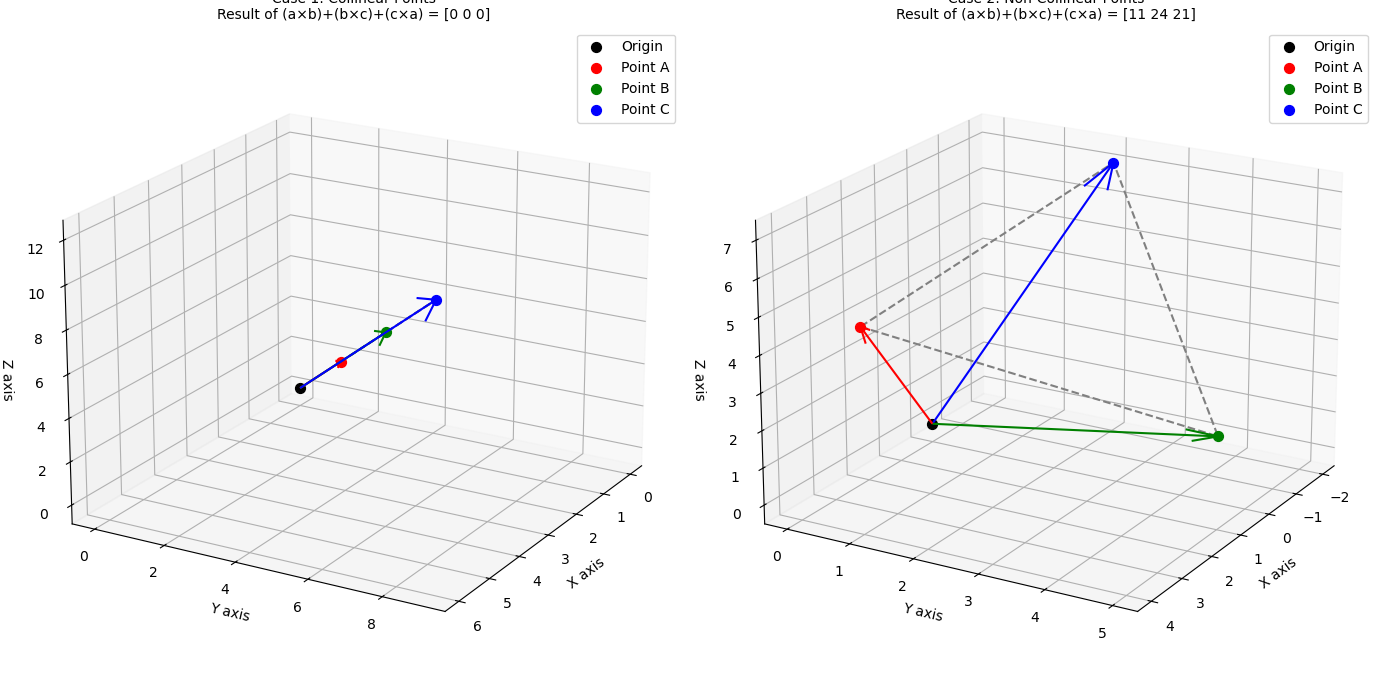
\includegraphics[width=\columnwidth, height=0.8\textheight, keepaspectratio]{figs/fig1.png}     
\end{frame}


\end{document}
